%% LaTeX2e class for student theses
%% sections/methodology.tex
%% 
%% Karlsruhe Institute of Technology
%% Institute for Program Structures and Data Organization
%% Chair for Software Design and Quality (SDQ)
%%
%% Dr.-Ing. Erik Burger
%% burger@kit.edu
%%
%% Version 1.3.6, 2022-09-28

\chapter{Methodology}
\label{ch:Methodolody}

%% -------------------
%% | Example content |
%% -------------------
Since our continual learning approach is, to the best of our knowledge, the first approach to combine pool-based active learning with continual
learning, we explain our approach in detail in this chapter as well as the motivation for it. We then transfer our approach to the domain of model
stealing. Because we build upon the framework of ActiveThief, we describe how our approach compares to the original approach in detail.

\section{Continual Active Learning}
\label{sec:Methodology:ContinualActiveLearning}
A major contribution of this thesis is that we combine the two learning paradigms of continual learning and active learning. To motivate the idea of
combining Continual Learning and Active Learning, we will first outline the classic Continual Learning Setting and the classic Active Learning Setting.
Next we explain common issues with these two learning paradigms and how we aim to overcome these by combining both paradigms. Finally, we will give
a detailed description of our approach. 

\subsection{The classic Continual Learning Setting}
\label{sec:Methodology:CLSetting}
%Mention that CL Setting consists of multiple tasks, task can and usually are independent
% Outline classic Continual Learning Workflow with a figure
In the typical continual learning setting, the model is trained on a sequence of tasks. Each task $T_i = {x_k,y_k | k \in \{1,\ldots,n\}}$ is a set of instances 
with their respective label. Together, the tasks form a dataset $D = \bigcup\limits_{i=1}^{N} T_i$. It is important to note that
the distribution of two distinct tasks $P(T_i)$  and $P(T_j) (i \neq j)$ are not necessarily the same. Most often in fact, the tasks are independent of each
other, which is why neural networks struggle to perform well on multiple tasks at once. This also means that the size of two distinct datasets can be
different, i.e. $|T_i| \neq |T_j|$ and so can the number of classes $|{y_k | \exists x_k: x_k,y_k \in T_i}| \neq |{y_l | \exists x_l: x_l,y_l \in T_j}|$.
When training a model on a sequence of tasks, the model is first fed with the data of the first task $T_1$ and then trained on it. After the model has been trained
on the first task, it can either be trained on the next task or deployed to classify samples stemming from the distribution of the first task. Next, the model is
trained on the second task. After being trained on the second task, the model should now be able to classify samples from the distribution of the first task as well
as the second task. This process is repeated until the model has been trained on all tasks. After being trained on all tasks, the model should be able to classify
%samples following the distribution of all the tasks it was trained on. This workflow is illustrated in Figure \ref{fig:CLWorkflow}. \\
The main difference between the continual learning setting and classic machine learning is that in the classic machine learning setting, the model is never retrained
once it is deployed. In the continual learning setting however, the model is retrained whenever a new task arrives.

\begin{figure}[ht]
    \centering
    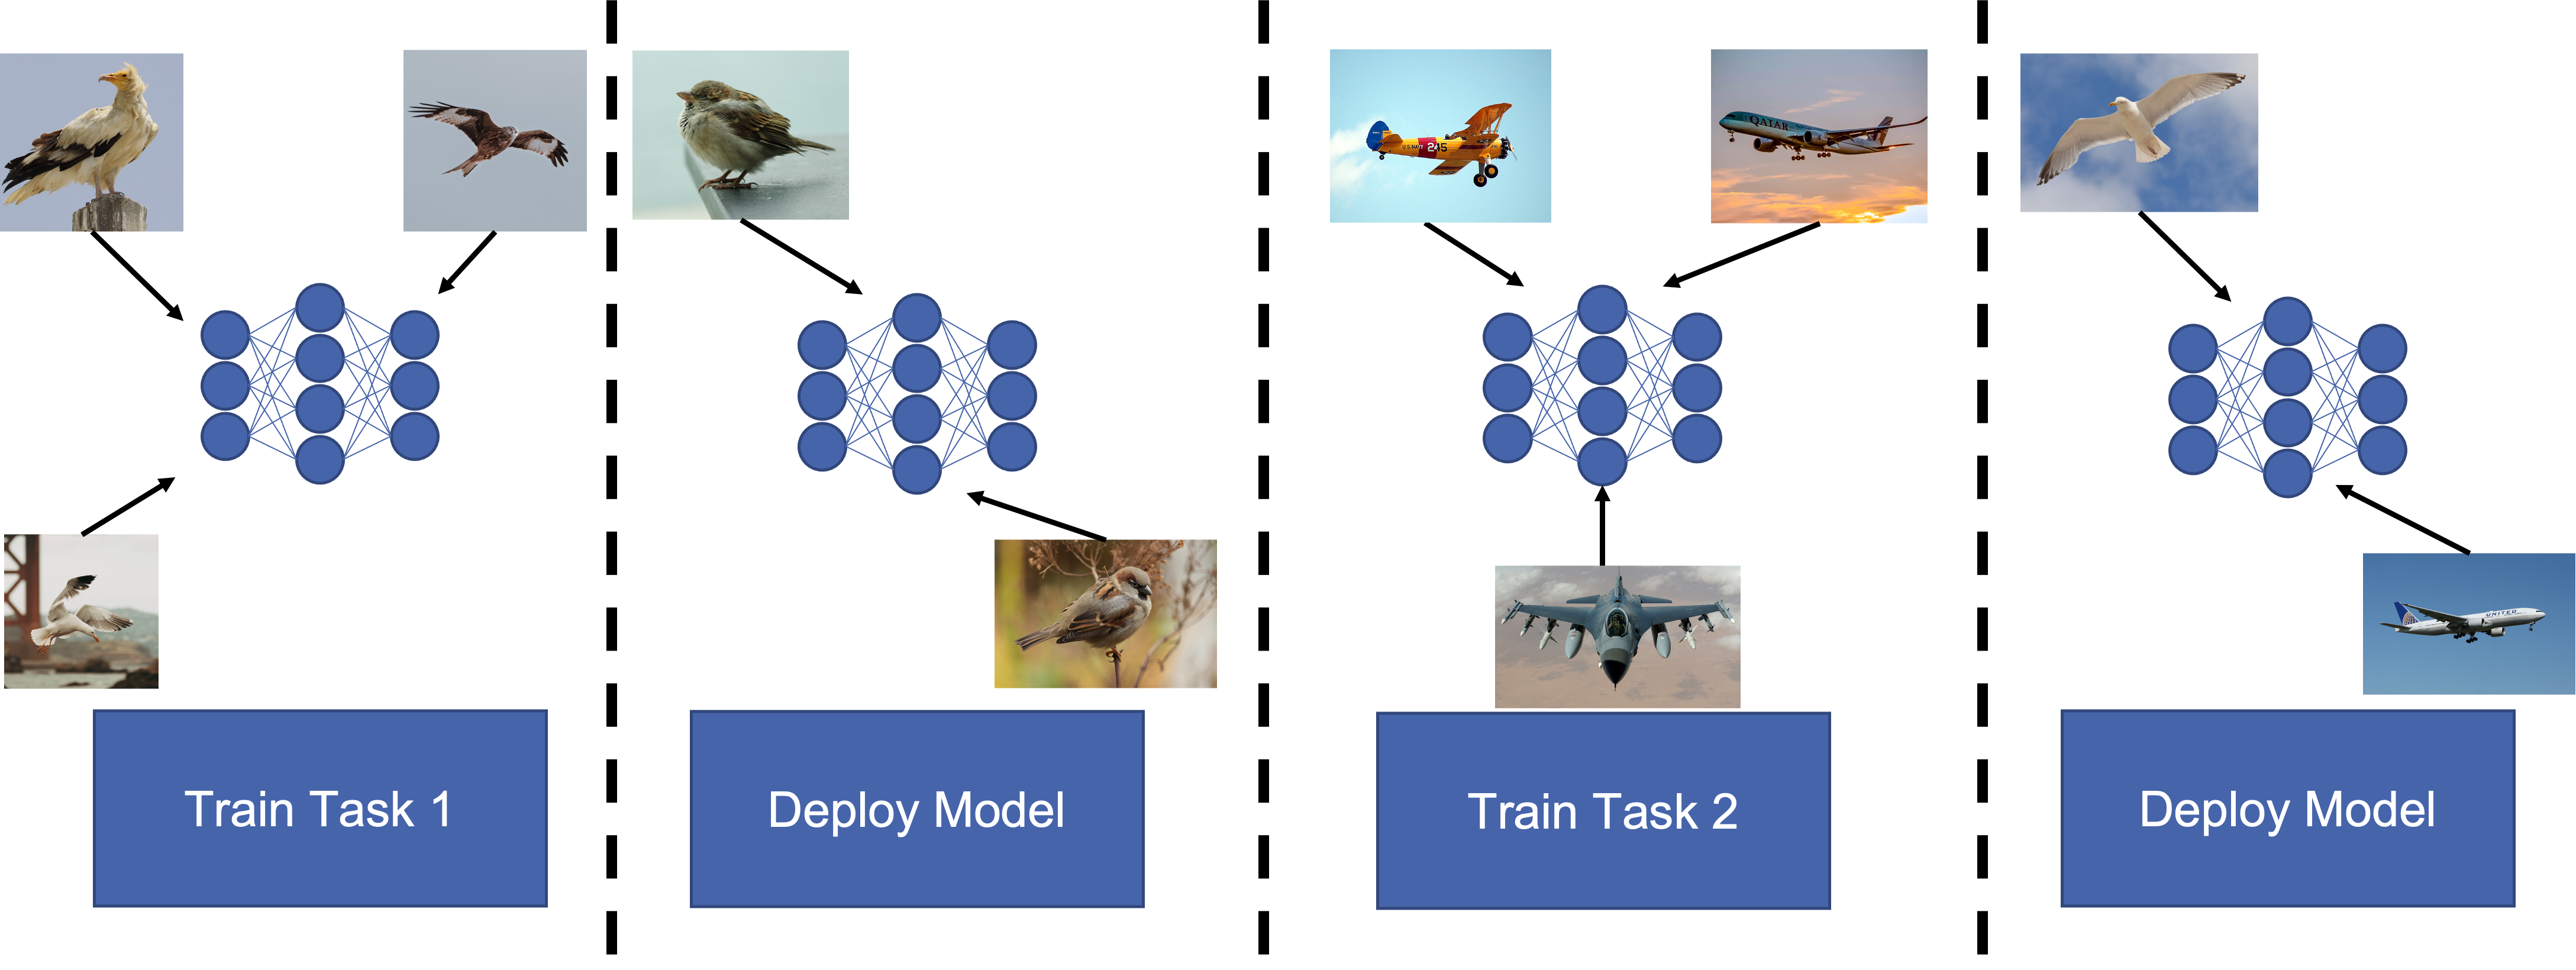
\includegraphics[width=.9\linewidth]{images/CL_workflow.png}
    \caption[Continual Learning Workflow]{Example for the classic Continual Learning Workflow. In this example, the model is first trained on different species of
    birds. It is then deployed to differentiate these species. Next, the model is trained on planes. After being deployed again, the model should now differentiate
    the planes as well as the birds.}
    \label{fig:CLWorkflow}
  \end{figure}

\subsection{The classic Active Learning Setting}
\label{sec:Methodology:ALSetting}
%TODO: Write this section
%Mention classic pool-based Active Learning setting, what batches are, contrast the continual
% learning setting, saying that the "tasks" are not independent

\subsection{Combining Continual and Active Learning}
% Mention the issues with the classic CL and AL setting, describe how synergising the two approaches
% can help overcome these issues and describe the approach in detail
\label{sec:Methodology:CombiningCLandAL}
The problem with classic Active Learning is that it is very resource intensive. When training a model using pool-based Active Learning on a dataset of size $n$,
with batch size $b$, the model will be trained $\frac{n}{b}$ times on the current labeled pool, equating to $\frac{n(n+b)}{2b}$ data points overall (we provide a
short derivation of this number in \ref{sec:appendix:FirstSection}). The problem with the number of data points used for training is that it is dependent on the
batch size $b$. The smaller the batch size, the larger the overall number of data points that the model is trained on. In the extreme case of $b=1$, the model
is trained on $\frac{n(n+1)}{2}$ data points. While \cite{beck2021effective} note that the batch size has a negligible effect on the performance of the model,
if any, a typical batch size is less than 10 \% of the full training set. Even in this more realistic case, the model is trained on $5.5n$ data points. When
comparing this to the classic Continual Learning setting, where the model is trained once using $n$ data points, it is clear to see that Active Learning comes
with a considerable overhead. The overhead of Active Learning is even more pronounced when considering the running time of the Active Learning Algorithms.
For more details we refer to the TODO experimental sections. \par
On the other hand, a major problem with classic Continual Learning is that task-ordering has a significant impact on the performance of the model \cite{bell2022effect}.
The problem of task-ordering has been studied before, and it has been shown that training samples in decreasing order of difficulty results in faster learning and 
improved generalization error \cite{hacohen2019power}. This motivates us to use Active Learning as a tool to perform task-ordering. We should note here that We
assume free choice of the next task. This assumption is not always realistic, especially when tasks arrive sequentially, but studying the effect of task-ordering
benefits the study of these scenarios, too. Furthermore, insights in the field of task-ordering help towards a more rigorous evaluation of continual learning in 
research because they allow to assess the influence of task-ordering on experiment results when using classic benchmark datasets. \par
Our approach aims to overcome both the issue of the overhead of Active Learning and the issue of task-ordering by combining both learning paradigms. We modify the Active
Learning process by training only on the currently selected batch instead of the entire labeled pool. This way, the model is trained on $\sum_{i=1}^{\frac{n}{b}} b = n$ 
data points, which fully eliminates the overhead of Active Learning from a data-centric perspective. Nevertheless, the query time of the Active Learning Algorithm remains
as an overhead. From a Continual Learning perspective, we join all tasks to a single dataset and use this dataset as the unlabeled pool for Active Learning. In each iteration
of the Active Learning process, we select a batch $B$ of data points from the unlabeled pool using the given Active Learning Strategy. This batch is then labeled by the
oracle if the initial dataset was unlabeled. If the initial dataset is labeled, we omit querying the oracle because the label is already known and simply add the labels
to the respective data points. We then treat the current batch $B$ as a new task and train our model using only the data points of $B$ with the Continual Learning strategy of
choice. This process is repeated until the unlabeled pool is empty. The full algorithm is described in Algorithm \ref{alg:PoolBasedContinualActiveLearning} where we high-
list the difference between classic pool-based Active Learning and our new Continual Active Learning approach in red. \par
%TODO: Mention here that we aim to increase the efficiency of the training process, i.e. we save time because we train on less
% data points

\begin{algorithm}
    \caption{Pool-based Continual Active Learning} \label{alg:PoolBasedContinualActiveLearning}
    \begin{algorithmic}[1]
        \Require Unlabeled data $U$,Labeled data $L = \emptyset$:, Oracle $O$, Model $M$, budget $B$
        \State Select $k$ data points from $U$ at random, obtain labels by querying $O$ and set $L=\{x_1,\ldots,x_1\}$
        and $U = U \setminus \{x_1,\ldots,x_1\}$ \Comment{Initialization}
        \State Train $M$ on initial labeled set $L$
        \While{label budget $B$ not exhausted}
            \State Select $l$ data points from $U$ predicted to be the most informative by the Active Learning strategy
            \State Obtain labels $y_i,\ldots,y_l$ by querying $O$ for $x_i,\ldots,x_l$
            \State {\color{red} Train $M$ on current labeled batch $\{(x_iy_i),\ldots,(x_l,y_l)\}$}
            \State Set $L= L \cup \{x_i,\ldots,x_l\}$ and $U = U \setminus \{x_i,\ldots,x_l\}$
            \State Train $M$ on labeled set $L$
        \EndWhile
    \end{algorithmic}
\end{algorithm}

\section{Continual Active Learning for Model Stealing}
\label{sec:Methodolody:CALMS}
% Transition to model stealing and elaborate why the continual active learning approach is interesting
% in the model stealing domain. Explain how the continual active learning approach has to be modified
% to apply it to model stealing. Best use a figure similar to the figure explaining the CAL approach
% and highlight the parts that are different
In this section, we describe how we apply the Continual Active Learning approach to the problem of model stealing. Using the Continual Active Learning approach
in the model stealing domain allows us to figure out, if the Continual Active Learning achieves a similar performance in the model stealing domain compared to
the standard setup where the oracle returns truthful labels. To motivate transferring our approach to the Active Learning domain, it is crucial to highlight the
differences between the setup mentioned in \ref{sec:Methodology:CombiningCLandAL} and Continual Active Learning for Model Stealing. \par
The first difference is that the labels returned by the oracle in the model stealing domain have a limited semantic meaning. This is because the oracle is another
machine learning model in the model stealing domain. So even if the data point whose label is queried stems from the same distribution as the target model dataset,
the label returned by the oracle is not necessarily correct since Machine Learning Models are not capable of generalizing perfectly. Since the target model dataset
is unknown to the attacker, he or she cannot knowingly construct a thief dataset that overlaps with the target model dataset. Therefore, the data points that the
attacker queries the target model with will most likely be from a different distribution than the target model dataset and the labels returned by the target model
will be incorrect. The example in Figure \ref{fig:CalmsWorkflow} highlights the meaning of the associated label. In the given example, the target model is trained
to classify planes which is why it associates the label \enquote{Fighter Jet} with a sparrow. \par
The second difference between the standard Continual Active Learning approach and Continual Active Learning for Model Stealing lies again in the labels returned by
the oracle. In the standard Continual Active Learning approach, the labels of the oracle are not only truthful, but the label is just a single value, i.e. the respective
class. In the model stealing domain, the label returned by the oracle is either a single value or the per-class probabilities of the output layer of the target model.
The latter is the more interesting case for Continual Active Learning because it reveals much more information about the function learned by the target model. \par
After explaining the motivation for applying the Continual Active Learning approach to the model stealing domain, we now describe how Continual Active Learning can be
applied for model stealing. The first step is to use the thief dataset as the initial unlabeled pool for Active Learning. The thief dataset is used by the Active Learning
strategy in each iteration as it would have been done in classic Continual Active Learning. After selecting the most informative samples to label, the target model is
queried for the labels of the selected samples. The label returned, which is either a single value or the per-class probabilities of the output layer of the target model,
is then used as the label of the respective data point that was queried throughout the whole training process. This means specifically that the gradient updates during 
training are based on the loss computed with a softmax label, allowing for a more fine-grained optimization of the weights to approximate the target model function. This
process is then repeated until the unlabeled pool is empty. A visual example of the Continual Active Learning for Model Stealing workflow is shown in Figure
\ref{fig:CalmsWorkflow}. \par
\begin{figure}[ht]
    \centering
    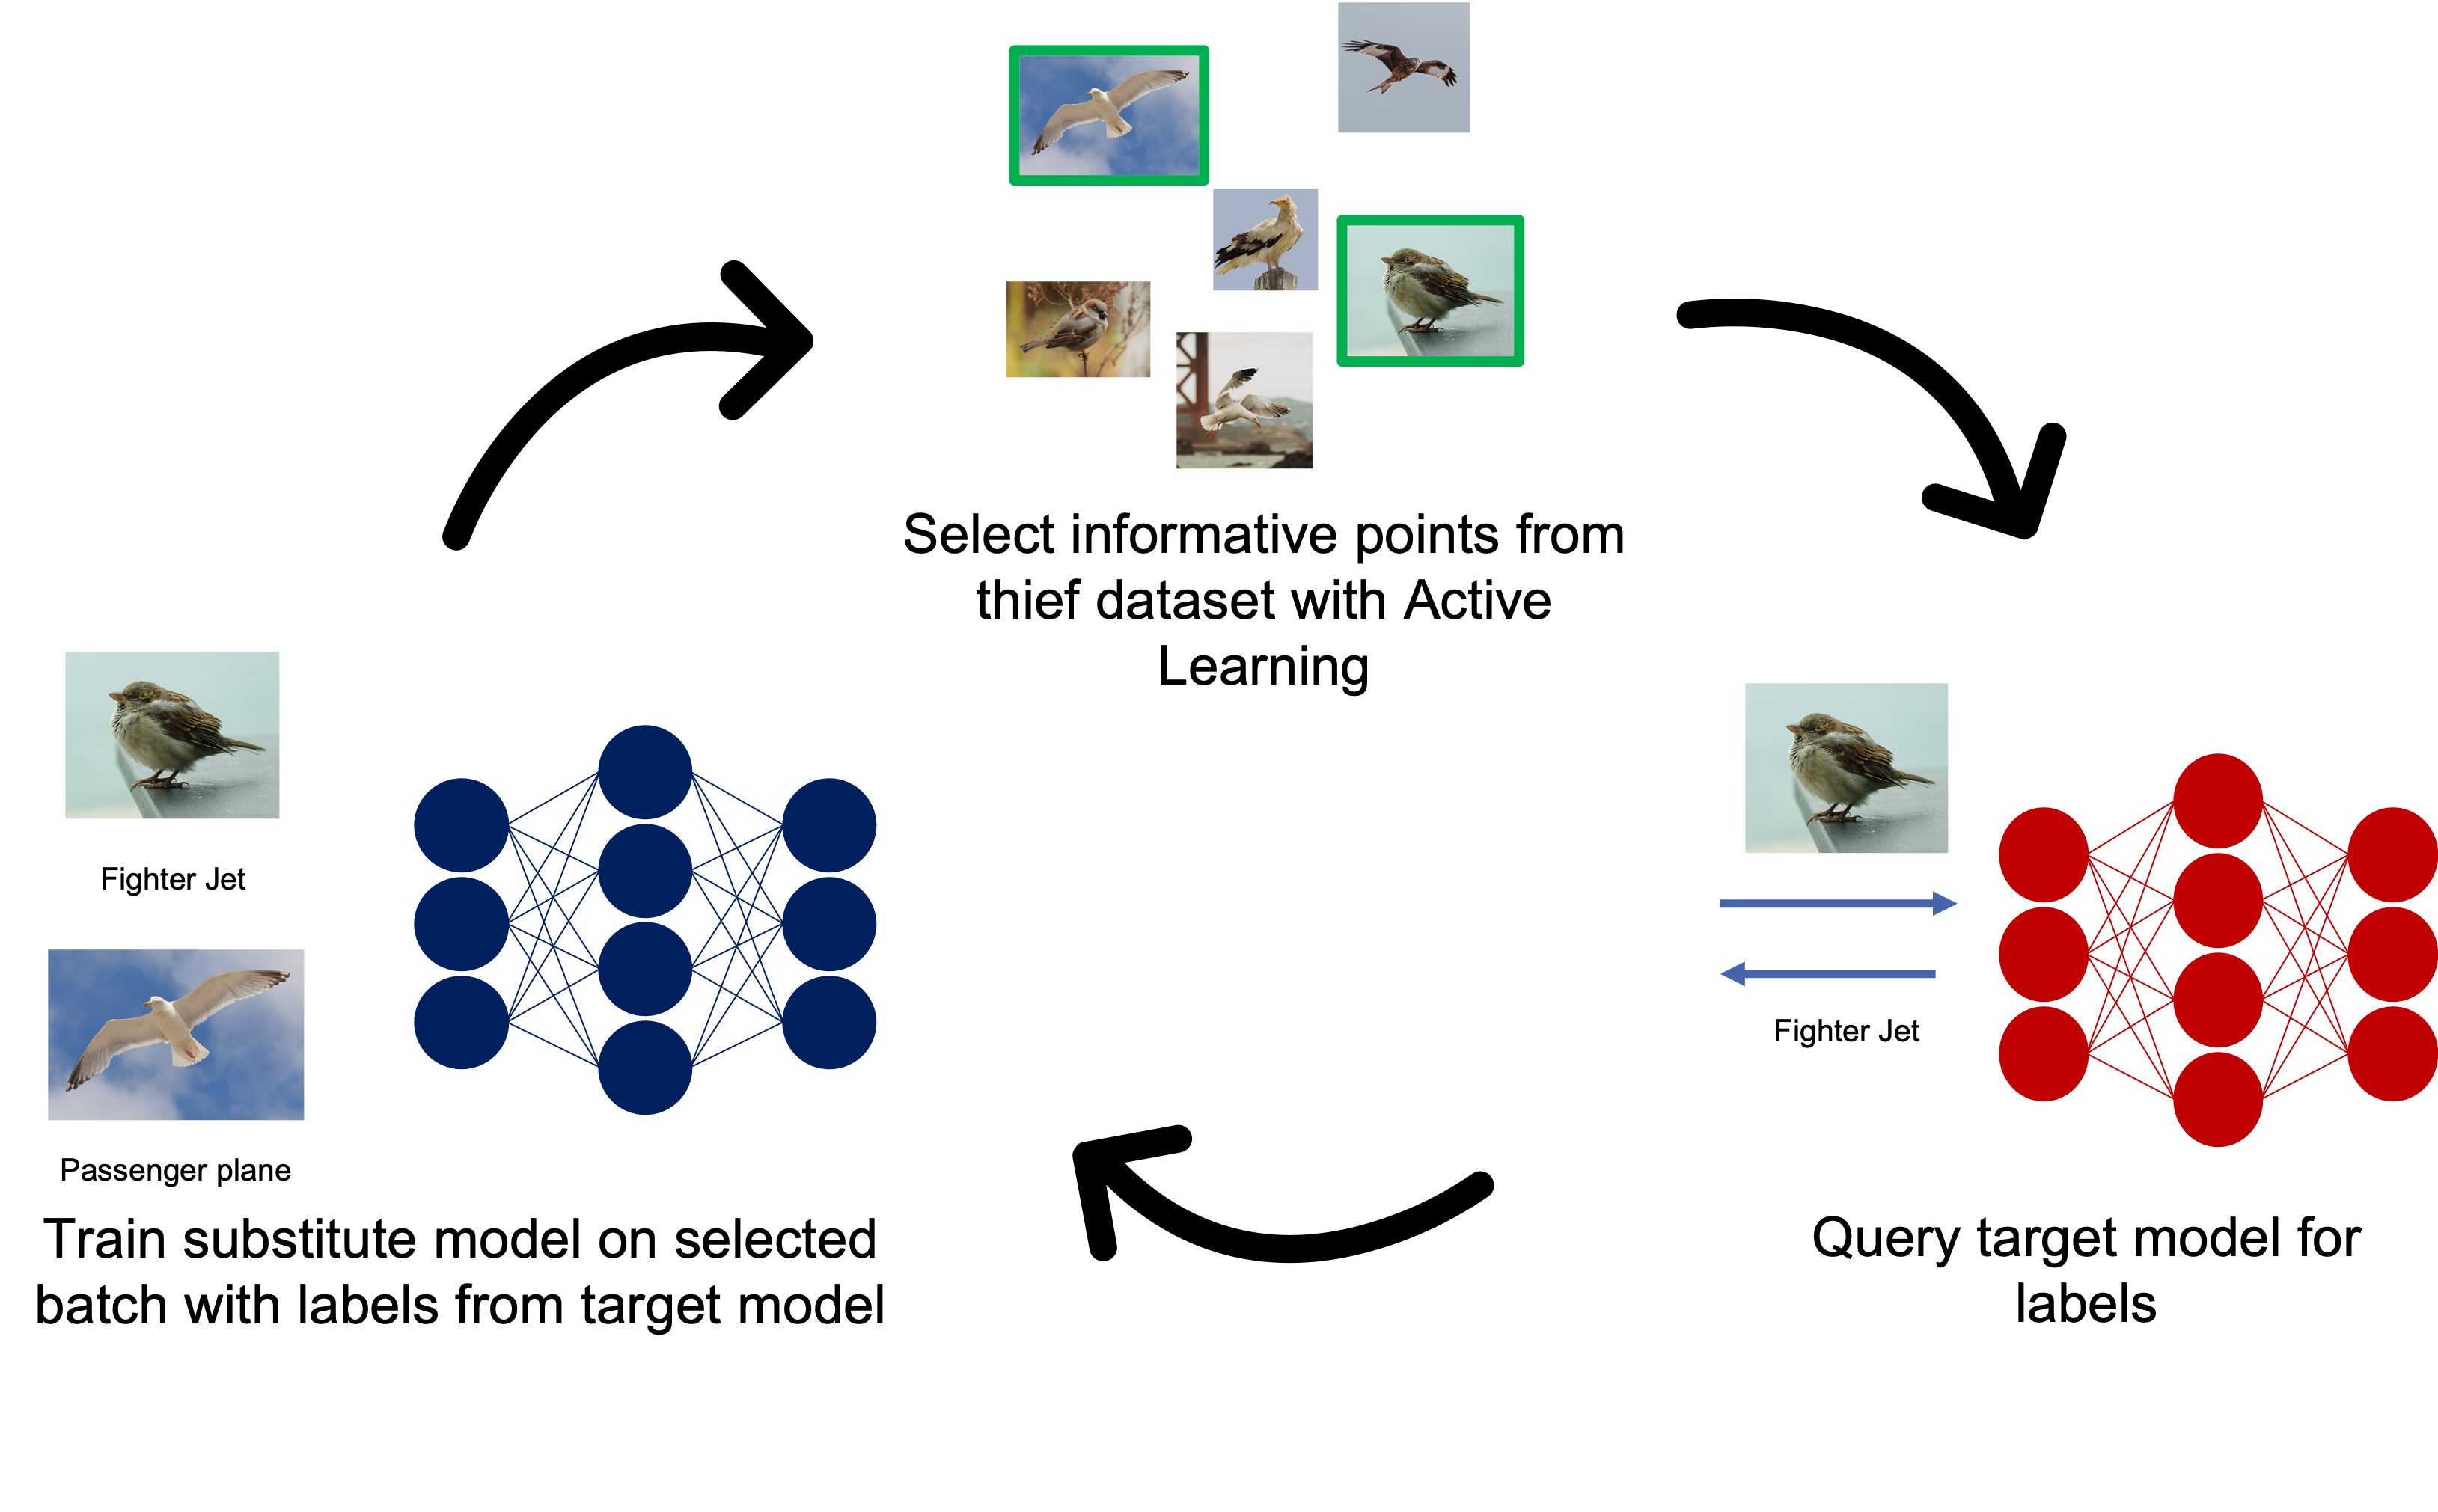
\includegraphics[width=.9\linewidth]{images/Calms_workflow.png}
    \caption[Continual Active Learning for Model Stealing Workflow]{Example of the Continual Active Learning for Model Stealing Workflow. In this example, the thief
    dataset consists of birds while the target model was trained to classify planes. In each iteration, a batch of informative samples is selected by the Active Learning
    strategy first. Next, the target model is queried for the labels of the selected samples. Since our thief dataset is composed of NNPD data, the associated labels have
    an incorrect semantic meaning. The thief model is then trained only on the selected samples from the current batch. This process is repeated iteratively.}
    \label{fig:CalmsWorkflow}
\end{figure}

\section{Replay strategy}
\label{sec:Methodology:ReplayStrategy}
In this section we propose a Continual Learning Strategy called Replay. Applying replay to overcome catastrophic forgetting is not an entirely new idea. In fact, it
has been proposed since the 1990s \cite{robins1995catastrophic}. The approach we propose modifies the classic replay by compressing the replay buffer. To understand the modification
we must first understand the classic replay strategy. \par
Replay is a Continual Learning strategy that stores a subset (or all) data points from each task in a so-called replay buffer. When training on a new task $T_N$, the model is trained 
on all data from the current task plus a sample from the replay buffer. After training on task $T_N$, the replay buffer is then updated with the data points from the current task. \par
A significant drawback of the classic Replay strategy is that the replay buffer can grow very large over time. This is especially true when the replay buffer stores all data points from
each task. It is much more desirable to have a Continual Learning strategy with a fixed memory footprint, because this reflects the realistic application of Continual Learning where memory 
is limited. \par
The proposed modification of the Replay strategy is to compress the replay buffer after each task. Assume we have a replay buffer of size $n$. After training on task $T_N$, the replay buffer
is combined with the data points from the current task to form a new set of data points $P$. We then select $n$ data points from $P$ to form the new replay buffer. The selection of the $n$ data
is done by performing one iteration of the Active Learning strategy CoreSet \cite{sener2018active} with $P$ as the unlabeled pool and $n$ as the batch size. The $n$ data points selected by Core-
Set then represent the new replay buffer. When training on task $T_{N+1}$, the model is trained on all data from the current task plus the full replay buffer.

%% ---------------------
%% | / Example content |
%% ---------------------